\documentclass{standalone}
\usepackage{tikz}
\usetikzlibrary{shapes.geometric, arrows, positioning, fit}

\begin{document}
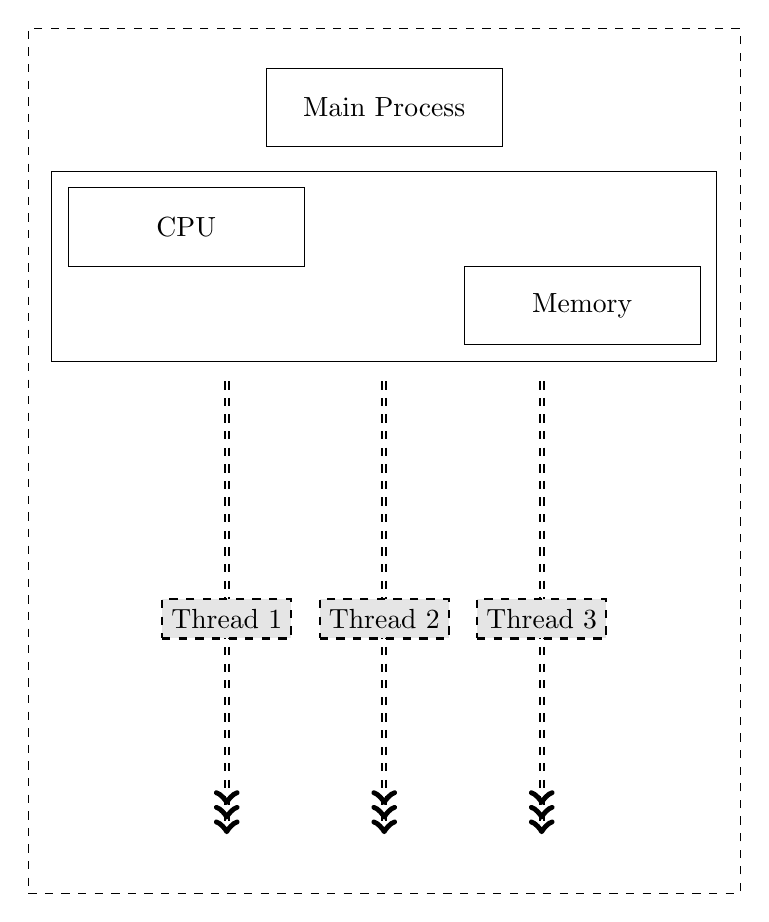
\begin{tikzpicture}[
    process/.style={rectangle, draw, minimum width=3cm, minimum height=1cm},
    thread/.style={rectangle, draw, minimum width=1cm, minimum height=0.5cm, fill=gray!20},
    arrow/.style={-latex, thick},
    dashedarrow/.style={->>>, double,thick, dashed},
    label/.style={font=\large\bfseries}
]

% Multithreading
\node[process] (main2) {Main Process};
\node[process, below right=1.5cm and -0.5cm of main2] (memory2) {Memory};
\node[process, below left=0.5cm and -0.5cm of main2] (cpu2) {CPU};

% Box around CPU and Memory in Multithreading
\node[draw, fit=(cpu2) (memory2), inner sep=0.2cm] (multithreading_cpu_mem) {};

% Threads
\node[below=0cm of multithreading_cpu_mem, xshift=-2cm] (thread1top) {};
\node[below=0cm of multithreading_cpu_mem] (thread2top) {};
\node[below=0cm of multithreading_cpu_mem, xshift=2cm] (thread3top) {};

\node[below=6cm of multithreading_cpu_mem, xshift=-2cm] (thread1bottom) {};
\node[below=6cm of multithreading_cpu_mem] (thread2bottom) {};
\node[below=6cm of multithreading_cpu_mem, xshift=2cm] (thread3bottom) {};

\draw[dashedarrow] (thread1top) -- (thread1bottom) node[thread, below=3cm of multithreading_cpu_mem,xshift=-2cm] {Thread 1};
\draw[dashedarrow] (thread2top) -- (thread2bottom) node[thread, below=3cm of multithreading_cpu_mem] {Thread 2};
\draw[dashedarrow] (thread3top) -- (thread3bottom) node[thread, below=3cm of multithreading_cpu_mem,xshift=2cm] {Thread 3};


% % Box around the entire multithreading section
\node[draw, dashed, fit=(main2) (cpu2) (memory2) (thread1bottom) (thread2bottom) (thread3bottom), inner sep=0.5cm] (multithreading) {};

\end{tikzpicture}
\end{document}